
%% %%
%% %% INTRO
%% %%

\slide{ Summary of recent updates }
{
wmunu version: v6: (3 weeks ago)
\iteb
\item Switched from mu18\_MG (buggy) to mu18 trigger
\item Increased number of MC toys (for SFs) from 100 to 1000
\itee
wmunu version: v7: (1 week ago)
\iteb
\item Fixed a bug that treated uncorrelated portion of QCD uncertainty as correlated
\item Added full difference between MET and W\_mT fits to QCD systematics
\item Wpt systematic updated to sum-in-quadrature of Sherpa14MC11 and PowhegPythia8MC11
\itee
wmunu version: v8: (\red{new})
\iteb
\item Cross-check: pileup uncertainty (scaling $<mu>$ by 0.97)
\item New source of QCD uncertainty: difference in DtoM fit vs (DtoK+LtoM)
\itee
Extra: a quick look at the toyMC uncertainty in Wmunu channel.
}

\slide{ QCD studies }
{
Recall that in the Wenu case, Adrian saw 20\% effects on QCD estimation from \red{MET vs mT} fits and from \red{DtoK+LtoM vs DtoM} fits.
}

\slide{ Adrian's plot: single-differential wenu ($pt>25$ GeV)}
{
\colb[T]
\column{.5\textwidth}
\centering
\small{ $W^{-}$: wenu}
\includegraphics[width=1.0\textwidth]{/home/antonk/SupportingDocument/Wenu/figures/uncert/with_theory/Wenu_Unc_neg}
\column{.5\textwidth}

\centering
\small{ $W^{+}$: wenu}
\includegraphics[width=1.0\textwidth]{/home/antonk/SupportingDocument/Wenu/figures/uncert/with_theory/Wenu_Unc_pos}
\cole
}

\slide{ wmunu: single-differential uncertainties ($pt>25$ GeV) }
{
\colb[T]
\column{.5\textwidth}
\centering
\only{ \small{ $W^{-}$: wmunu v8} }
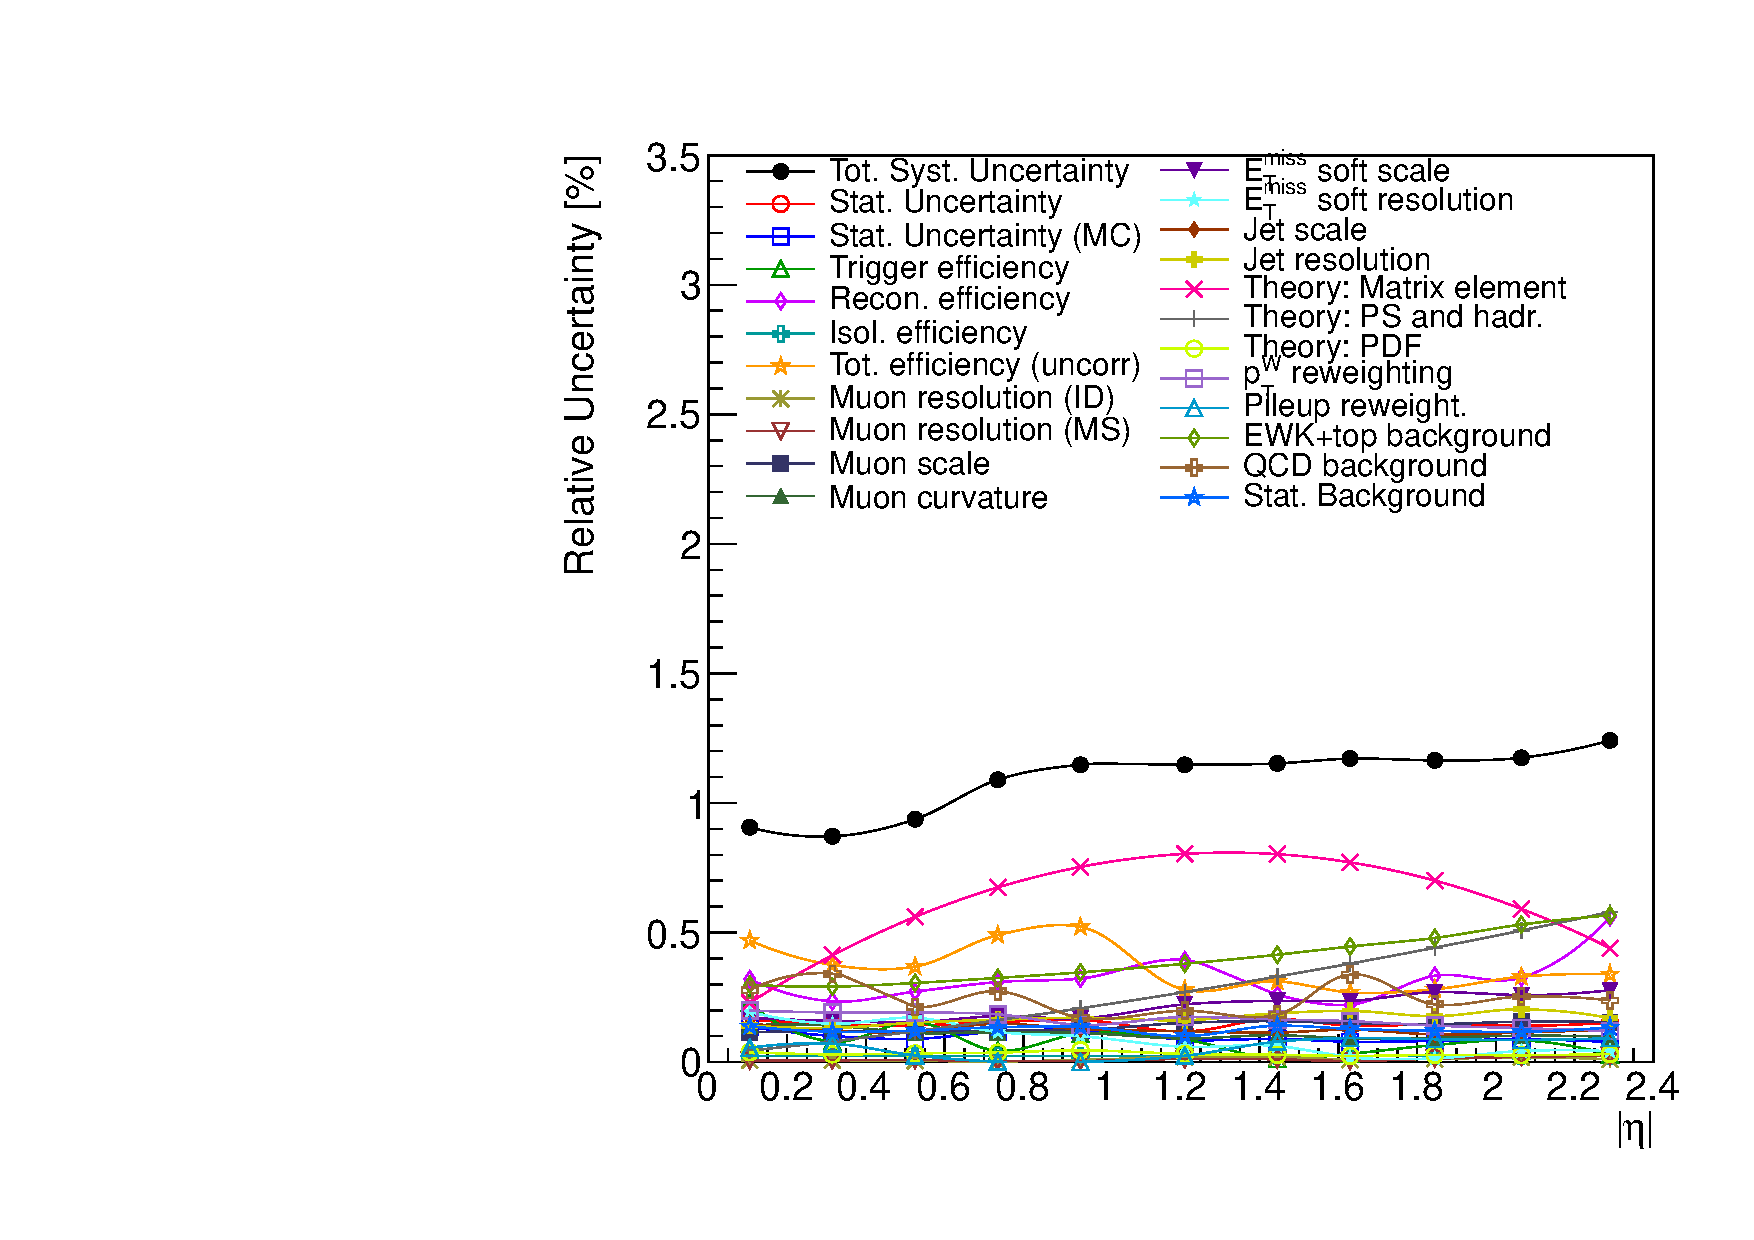
\includegraphics[width=1.0\textwidth]{dates/20130602/figures/v26.allqcd/Wmn_SYSTEM_1D_PT25_NEG_Unc_proj}
\column{.5\textwidth}

\centering
\only{ \small{ $W^{+}$: wmunu v8} }
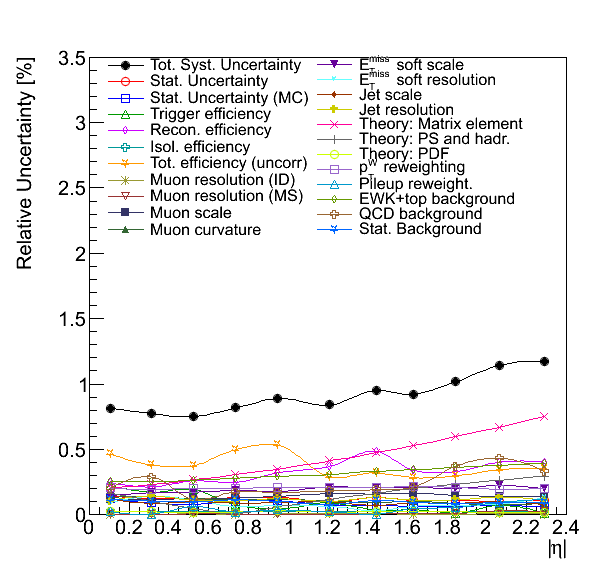
\includegraphics[width=1.0\textwidth]{dates/20130602/figures/v26.allqcd/Wmn_SYSTEM_1D_PT25_POS_Unc_proj}
\cole
}

\slide{ Comment }
{
I see smaller bin-by-bin fluctuations in QCD uncertainties in the wmunu channel. \\
Let's see what happens in the case of a lowered pT cut.
}

\slide{ Single-differential uncertainties ($pt>20$ GeV) }
{
\colb[T]
\column{.5\textwidth}
\centering
\only{ \small{ $W^{-}$: wmunu v8} }
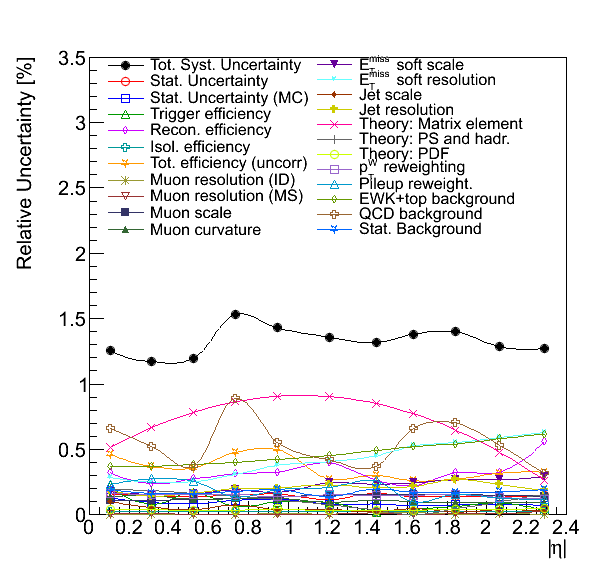
\includegraphics[width=1.0\textwidth]{dates/20130602/figures/v26.allqcd/Wmn_SYSTEM_1D_PT20_NEG_Unc_proj}
\column{.5\textwidth}

\centering
\only{ \small{ $W^{+}$: wmunu v8} }
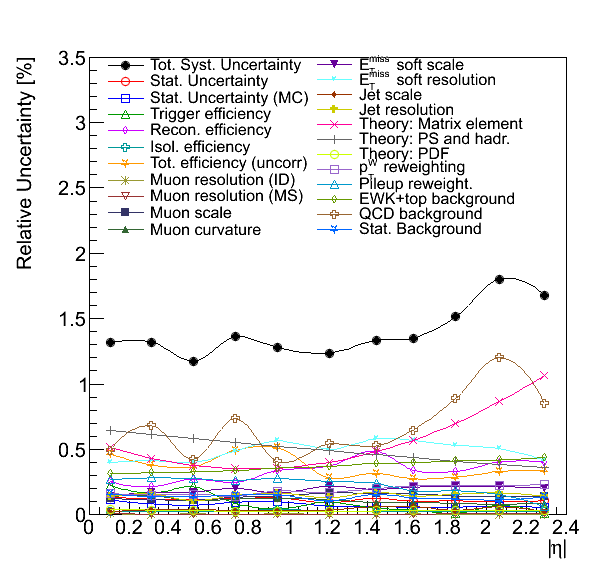
\includegraphics[width=1.0\textwidth]{dates/20130602/figures/v26.allqcd/Wmn_SYSTEM_1D_PT20_POS_Unc_proj}
\cole
}

\slide{ Comment }
{
QCD uncertainty (driven by MET vs Wmt) is more significant with a 20 GeV cut. \\
It's probably better to focus on the measurement with a 25 GeV cut and extrapolate. \\

Also note that the additional pileup uncertainty from $<mu>$ scaling is negligible in
single-differential case. In the backup, I show all double-differential plots. This pileup
scaling is only appreciable in the lowest pt bin (20-25 GeV), repeated on next slide.
}

\slide{ $20 < p_T < 25$ }
{
\colb[T]
\column{.5\textwidth}
\centering
\only{ \small{ $W^{-}$: wmunu v8} }
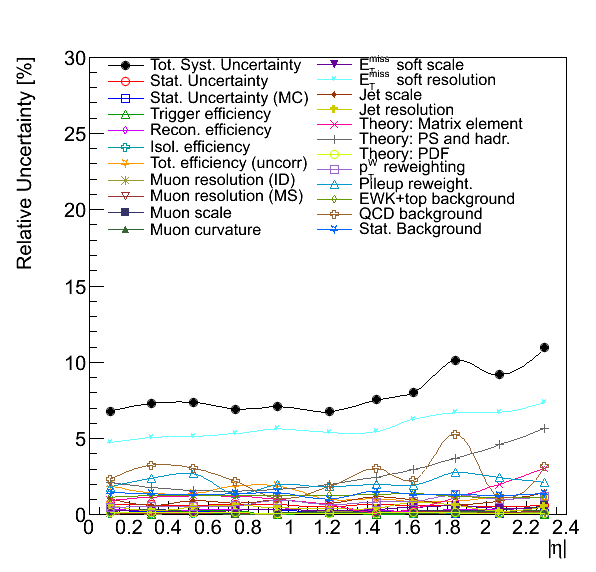
\includegraphics[width=1.0\textwidth]{dates/20130602/figures/v26.allqcd/Wmn_SYSTEM30_2D_PT20_NEG_Unc_2d_Slice_1}
\column{.5\textwidth}

\centering
\only{ \small{ $W^{+}$: wmunu v8} }
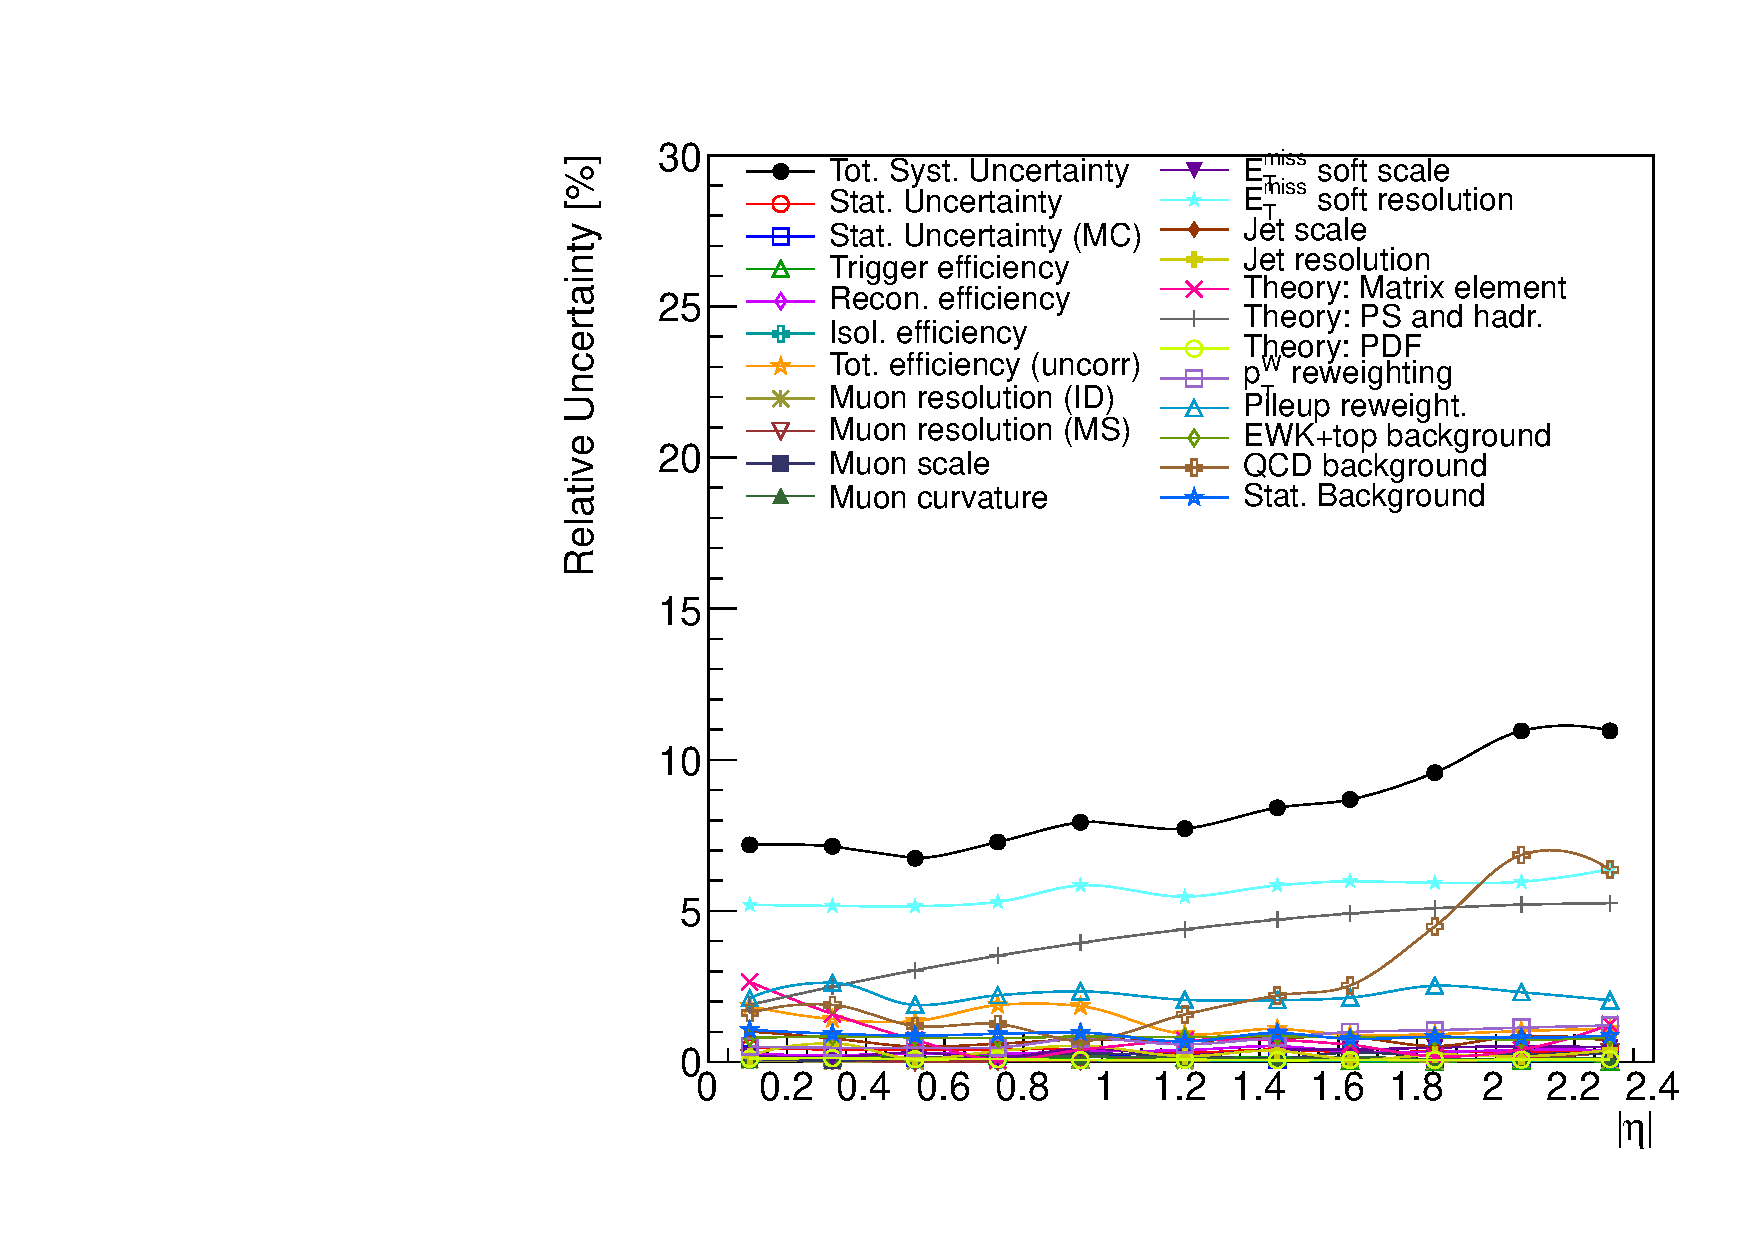
\includegraphics[width=1.0\textwidth]{dates/20130602/figures/v26.allqcd/Wmn_SYSTEM30_2D_PT20_POS_Unc_2d_Slice_1}
\cole
}

\slide{ Tables }
{
Let's quantify the additional pileup uncertainty, as well as various contributions to QCD uncertainty.
}

\slide{ Integrated $mu^+$, $pt>25$ GeV} 
{
\begin{table}
  \begin{center}
\tiny
    \begin{tabular}{lrr}
      \hline
      \hline
      Variation & $\delta \sigma_{W+}/\sigma_{W+}$ \\
      \hline

Trigger efficiency                       & 0.051 \\
Recon. efficiency                        & 0.336 \\
Isol. efficiency                         & 0.024 \\
Tot. efficiency (uncorr)                 & 0.110 \\
Muon resolution (ID)                     & 0.002 \\
Muon resolution (MS)                     & 0.004 \\
Muon scale                               & 0.141 \\
Muon curvature                           & 0.104 \\
$E_{T}^{miss}$ soft scale                  & 0.191 \\
$E_{T}^{miss}$ soft resolution             & 0.084 \\
Jet scale                                & 0.091 \\
Jet resolution                           & 0.107 \\
Theory: Matrix element                   & 0.412 \\
Theory: PS and hadr.                     & 0.194 \\
Theory: PDF                              & 0.090 \\
$p^{W}_{T}$ reweighting                    & 0.185 \\
\red{Pileup reweight.}                         & 0.017 \\
EWK+top background                       & 0.321 \\
\red{QCD: anti-isolation}                      & 0.095 \\
\red{QCD: fit range}                           & 0.122 \\
\red{QCD: fit variable}                        & 0.187 \\
\red{QCD: DtoK+LtoM}                           & 0.006 \\
Stat. Background                         & 0.030 \\
Stat. Uncertainty (MC)                   & 0.025 \\
\hline
Stat. Uncertainty                        & 0.035 \\
\hline
Tot. Syst. Uncertainty                   & 0.797 \\
      \hline
      \hline
    \end{tabular}
  \end{center}
\end{table}

}


\slide{ Integrated $mu^-$, $pt>25$ GeV} 
{
\begin{table}
  \begin{center}
\tiny
    \begin{tabular}{lrr}
      \hline
      \hline
      Variation & $\delta \sigma_{W-}/\sigma_{W-}$ \\
      \hline
Trigger efficiency                       & 0.037 \\
Recon. efficiency                        & 0.323 \\
Isol. efficiency                         & 0.023 \\
Tot. efficiency (uncorr)                 & 0.109 \\
Muon resolution (ID)                     & 0.003 \\
Muon resolution (MS)                     & 0.006 \\
Muon scale                               & 0.133 \\
Muon curvature                           & 0.104 \\
$E_{T}^{miss}$ soft scale                  & 0.209 \\
$E_{T}^{miss}$ soft resolution             & 0.073 \\
Jet scale                                & 0.120 \\
Jet resolution                           & 0.157 \\
Theory: Matrix element                   & 0.634 \\
Theory: PS and hadr.                     & 0.357 \\
Theory: PDF                              & 0.123 \\
$p^{W}_{T}$ reweighting                    & 0.146 \\
\red{Pileup reweight.}                         & 0.012 \\
EWK+top background                       & 0.401 \\
\red{QCD: anti-isolation}                      & 0.148 \\
\red{QCD: fit range}                           & 0.139 \\
\red{QCD: fit variable}                        & 0.037 \\
\red{QCD: DtoK+LtoM}                           & 0.004 \\
Stat. Background                         & 0.040 \\
Stat. Uncertainty (MC)                   & 0.029 \\
\hline
Stat. Uncertainty                        & 0.044 \\
\hline
Tot. Syst. Uncertainty                   & 1.003 \\

      \hline
      \hline
    \end{tabular}
  \end{center}
\end{table}

}

\slide{ Single-differential $mu^-$, $pt>25$ GeV} 
{
\begin{table}
  \begin{center}
\tiny
\begin{tabular}{l|p{0.6cm}p{0.6cm}p{0.6cm}p{0.6cm}p{0.6cm}p{0.6cm}p{0.6cm}p{0.6cm}p{0.6cm}p{0.6cm}p{0.6cm}}
\hline
   & 0.00, & 0.21, & 0.42, & 0.63, & 0.84, & 1.05, & 1.37, & 1.52, & 1.74, & 1.95, & 2.18,  \\ 
   & 0.21 & 0.42 & 0.63 & 0.84 & 1.05 & 1.37 & 1.52 & 1.74 & 1.95 & 2.18 & 2.40  \\ 
\hline
Trigger efficiency                       & 0.230 & 0.079 & 0.156 & 0.043 & 0.109 & 0.087 & 0.012 & 0.032 & 0.066 & 0.084 & 0.028 \\
Recon. efficiency                        & 0.320 & 0.234 & 0.272 & 0.309 & 0.322 & 0.393 & 0.259 & 0.222 & 0.333 & 0.326 & 0.560 \\
Isol. efficiency                         & 0.023 & 0.023 & 0.023 & 0.023 & 0.023 & 0.024 & 0.024 & 0.024 & 0.024 & 0.024 & 0.023 \\
Tot. efficiency (uncorr)                 & 0.469 & 0.375 & 0.369 & 0.490 & 0.522 & 0.279 & 0.311 & 0.269 & 0.281 & 0.330 & 0.339 \\
Muon resolution (ID)                     & 0.007 & 0.007 & 0.004 & 0.003 & 0.008 & 0.020 & 0.020 & 0.009 & 0.012 & 0.018 & 0.011 \\
Muon resolution (MS)                     & 0.006 & 0.007 & 0.008 & 0.004 & 0.004 & 0.012 & 0.010 & 0.004 & 0.013 & 0.020 & 0.025 \\
Muon scale                               & 0.114 & 0.121 & 0.115 & 0.122 & 0.124 & 0.151 & 0.157 & 0.149 & 0.146 & 0.156 & 0.154 \\
Muon curvature                           & 0.142 & 0.141 & 0.112 & 0.115 & 0.113 & 0.091 & 0.104 & 0.091 & 0.094 & 0.102 & 0.098 \\
$E_{T}^{miss}$ soft scale                  & 0.170 & 0.159 & 0.154 & 0.177 & 0.169 & 0.223 & 0.237 & 0.236 & 0.270 & 0.257 & 0.277 \\
$E_{T}^{miss}$ soft resolution             & 0.194 & 0.148 & 0.171 & 0.116 & 0.100 & 0.059 & 0.062 & 0.018 & 0.014 & 0.043 & 0.042 \\
Jet scale                                & 0.151 & 0.119 & 0.118 & 0.148 & 0.127 & 0.119 & 0.114 & 0.125 & 0.107 & 0.114 & 0.126 \\
Jet resolution                           & 0.142 & 0.132 & 0.152 & 0.163 & 0.171 & 0.161 & 0.188 & 0.197 & 0.177 & 0.204 & 0.169 \\
Theory: Matrix element                   & 0.229 & 0.412 & 0.560 & 0.674 & 0.753 & 0.804 & 0.802 & 0.771 & 0.701 & 0.591 & 0.440 \\
Theory: PS and hadr.                     & 0.044 & 0.080 & 0.119 & 0.162 & 0.207 & 0.270 & 0.330 & 0.380 & 0.441 & 0.508 & 0.579 \\
Theory: PDF                              & 0.038 & 0.030 & 0.034 & 0.037 & 0.046 & 0.031 & 0.028 & 0.024 & 0.028 & 0.026 & 0.031 \\
$p^{W}_{T}$ reweighting                    & 0.199 & 0.191 & 0.191 & 0.184 & 0.144 & 0.174 & 0.164 & 0.158 & 0.141 & 0.131 & 0.120 \\
\red{Pileup reweight.}                         & 0.055 & 0.071 & 0.026 & 0.001 & 0.001 & 0.024 & 0.079 & 0.093 & 0.088 & 0.085 & 0.092 \\
EWK+top background                       & 0.299 & 0.291 & 0.305 & 0.325 & 0.346 & 0.379 & 0.414 & 0.446 & 0.479 & 0.531 & 0.567 \\
\red{QCD: anti-isolation}                      & 0.185 & 0.151 & 0.130 & 0.108 & 0.086 & 0.118 & 0.161 & 0.182 & 0.136 & 0.239 & 0.124 \\
\red{QCD: fit range}                           & 0.153 & 0.118 & 0.166 & 0.194 & 0.103 & 0.148 & 0.085 & 0.163 & 0.158 & 0.056 & 0.160 \\
\red{QCD: fit variable}                        & 0.136 & 0.282 & 0.005 & 0.158 & 0.086 & 0.054 & 0.004 & 0.233 & 0.067 & 0.038 & 0.125 \\
\red{QCD: DtoK+LtoM}                           & 0.033 & 0.003 & 0.025 & 0.013 & 0.062 & 0.021 & 0.014 & 0.002 & 0.041 & 0.049 & 0.001 \\
Stat. Background                         & 0.138 & 0.117 & 0.122 & 0.134 & 0.137 & 0.101 & 0.140 & 0.128 & 0.120 & 0.117 & 0.134 \\
Stat. Uncertainty (MC)                   & 0.136 & 0.101 & 0.090 & 0.117 & 0.124 & 0.085 & 0.089 & 0.078 & 0.082 & 0.088 & 0.077 \\
\hline
Stat. Uncertainty                        & 0.164 & 0.146 & 0.142 & 0.154 & 0.162 & 0.118 & 0.166 & 0.140 & 0.146 & 0.140 & 0.152 \\
\hline
Tot. Syst. Uncertainty                   & 0.906 & 0.871 & 0.937 & 1.090 & 1.148 & 1.148 & 1.153 & 1.171 & 1.164 & 1.175 & 1.241 \\
\hline
\end{tabular}
  \end{center}
\end{table}

}


\slide{ Single-differential $mu^+$, $pt>25$ GeV} 
{
\begin{table}
  \begin{center}
\tiny
\begin{tabular}{l|p{0.6cm}p{0.6cm}p{0.6cm}p{0.6cm}p{0.6cm}p{0.6cm}p{0.6cm}p{0.6cm}p{0.6cm}p{0.6cm}p{0.6cm}}
\hline
   & 0.00, & 0.21, & 0.42, & 0.63, & 0.84, & 1.05, & 1.37, & 1.52, & 1.74, & 1.95, & 2.18,  \\ 
   & 0.21 & 0.42 & 0.63 & 0.84 & 1.05 & 1.37 & 1.52 & 1.74 & 1.95 & 2.18 & 2.40  \\ 
\hline
Trigger efficiency                       & 0.227 & 0.173 & 0.194 & 0.077 & 0.044 & 0.092 & 0.034 & 0.037 & 0.008 & 0.071 & 0.009 \\
Recon. efficiency                        & 0.248 & 0.213 & 0.261 & 0.246 & 0.321 & 0.370 & 0.485 & 0.341 & 0.330 & 0.403 & 0.401 \\
Isol. efficiency                         & 0.024 & 0.024 & 0.024 & 0.026 & 0.024 & 0.024 & 0.025 & 0.024 & 0.024 & 0.025 & 0.024 \\
Tot. efficiency (uncorr)                 & 0.469 & 0.382 & 0.376 & 0.497 & 0.534 & 0.290 & 0.323 & 0.283 & 0.298 & 0.345 & 0.351 \\
Muon resolution (ID)                     & 0.004 & 0.001 & 0.008 & 0.003 & 0.006 & 0.007 & 0.010 & 0.003 & 0.003 & 0.010 & 0.006 \\
Muon resolution (MS)                     & 0.004 & 0.002 & 0.007 & 0.006 & 0.003 & 0.006 & 0.006 & 0.011 & 0.009 & 0.030 & 0.023 \\
Muon scale                               & 0.116 & 0.114 & 0.127 & 0.128 & 0.140 & 0.162 & 0.159 & 0.166 & 0.150 & 0.139 & 0.142 \\
Muon curvature                           & 0.133 & 0.140 & 0.125 & 0.114 & 0.121 & 0.104 & 0.094 & 0.101 & 0.086 & 0.079 & 0.087 \\
$E_{T}^{miss}$ soft scale                  & 0.146 & 0.168 & 0.173 & 0.186 & 0.177 & 0.212 & 0.207 & 0.209 & 0.203 & 0.224 & 0.198 \\
$E_{T}^{miss}$ soft resolution             & 0.087 & 0.141 & 0.113 & 0.062 & 0.071 & 0.063 & 0.032 & 0.065 & 0.071 & 0.084 & 0.130 \\
Jet scale                                & 0.122 & 0.087 & 0.100 & 0.090 & 0.092 & 0.100 & 0.072 & 0.090 & 0.088 & 0.100 & 0.077 \\
Jet resolution                           & 0.105 & 0.141 & 0.112 & 0.105 & 0.123 & 0.103 & 0.131 & 0.112 & 0.114 & 0.135 & 0.110 \\
Theory: Matrix element                   & 0.205 & 0.233 & 0.267 & 0.305 & 0.349 & 0.412 & 0.475 & 0.528 & 0.596 & 0.671 & 0.753 \\
Theory: PS and hadr.                     & 0.165 & 0.103 & 0.045 & 0.009 & 0.060 & 0.118 & 0.165 & 0.198 & 0.233 & 0.265 & 0.293 \\
Theory: PDF                              & 0.024 & 0.022 & 0.019 & 0.021 & 0.031 & 0.021 & 0.022 & 0.022 & 0.022 & 0.018 & 0.018 \\
$p^{W}_{T}$ reweighting                    & 0.206 & 0.193 & 0.204 & 0.201 & 0.212 & 0.211 & 0.210 & 0.214 & 0.211 & 0.194 & 0.203 \\
\red{Pileup reweight.}                         & 0.026 & 0.006 & 0.063 & 0.021 & 0.037 & 0.022 & 0.005 & 0.048 & 0.053 & 0.093 & 0.120 \\
EWK+top background                       & 0.252 & 0.254 & 0.264 & 0.279 & 0.290 & 0.308 & 0.334 & 0.345 & 0.361 & 0.378 & 0.394 \\
\red{QCD: anti-isolation}                      & 0.141 & 0.117 & 0.087 & 0.077 & 0.063 & 0.080 & 0.107 & 0.117 & 0.084 & 0.115 & 0.058 \\
\red{QCD: fit range}                           & 0.125 & 0.116 & 0.071 & 0.118 & 0.086 & 0.159 & 0.140 & 0.116 & 0.132 & 0.115 & 0.126 \\
\red{QCD: fit variable}                        & 0.028 & 0.233 & 0.027 & 0.091 & 0.125 & 0.002 & 0.066 & 0.130 & 0.337 & 0.401 & 0.295 \\
\red{QCD: DtoK+LtoM}                           & 0.053 & 0.037 & 0.017 & 0.046 & 0.034 & 0.042 & 0.040 & 0.007 & 0.011 & 0.005 & 0.035 \\
Stat. Background                         & 0.119 & 0.105 & 0.098 & 0.115 & 0.103 & 0.079 & 0.108 & 0.093 & 0.089 & 0.091 & 0.091 \\
Stat. Uncertainty (MC)                   & 0.122 & 0.091 & 0.080 & 0.104 & 0.108 & 0.073 & 0.074 & 0.064 & 0.066 & 0.070 & 0.061 \\
\hline
Stat. Uncertainty                        & 0.141 & 0.125 & 0.121 & 0.131 & 0.135 & 0.096 & 0.132 & 0.110 & 0.112 & 0.104 & 0.112 \\
\hline
Tot. Syst. Uncertainty                   & 0.815 & 0.774 & 0.750 & 0.817 & 0.890 & 0.840 & 0.951 & 0.921 & 1.016 & 1.145 & 1.171 \\
\hline
\end{tabular}
  \end{center}
\end{table}

}

\slide{ Conclusions }
{
  QCD estimate seems robust against DtoK+LtoM vs DtoM fits, and against additional pileup uncertainty. \\
  Note that this pileup uncertainty should probably be excluded from final list of systematics, since it's largely already included in, e.g., MET uncertainty.
}



\slide{ Stat. uncertainty on scale factors: wmunu vs zmumu }
{
Uncorrelated SF uncertainty (from toy MCs) is fairly large in wmunu (but not zmumu): \\
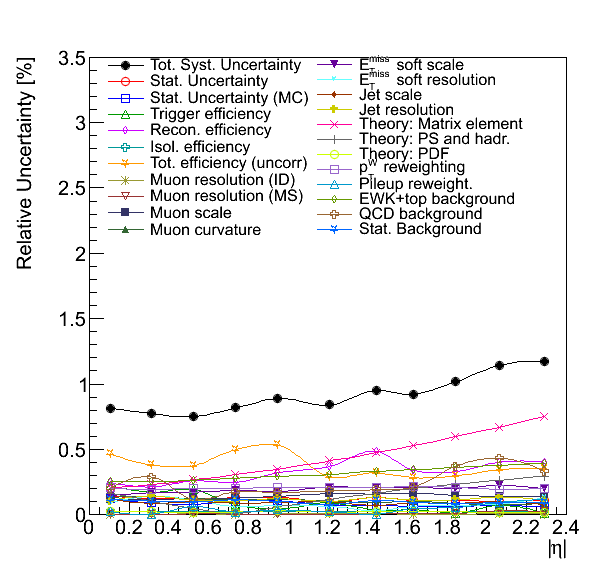
\includegraphics[width=0.5\textwidth]{dates/20130602/figures/v26.allqcd/Wmn_SYSTEM_1D_PT25_POS_Unc_proj}
}

\slide{ Also: stat. MC uncertainty looks problematic in fits }
{
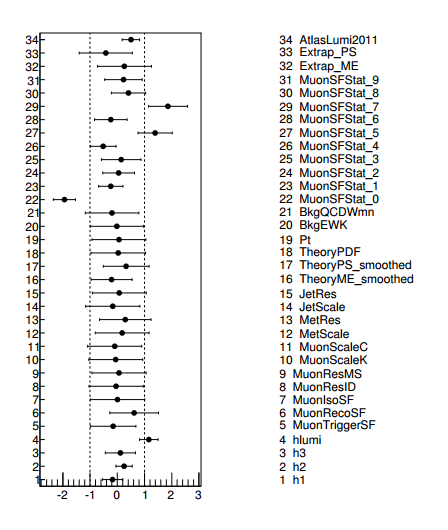
\includegraphics[width=0.4\textwidth]{dates/20130602/figures/fit/wmunu}
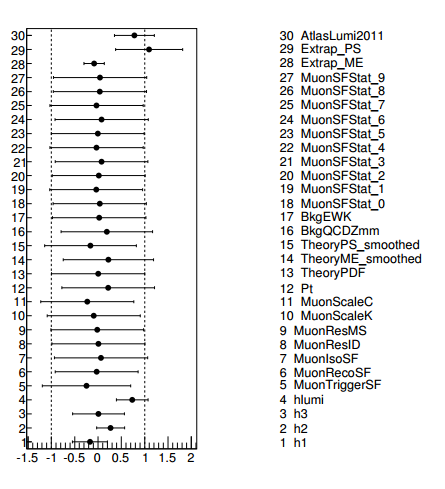
\includegraphics[width=0.4\textwidth]{dates/20130602/figures/fit/zmumu}
}

\slide{ What's responsible: reco, trigger, or isolation? }
{
\includegraphics[width=1.0\textwidth]<1>{dates/20130602/figures/toysf/EVENT_8701402}
\includegraphics[width=1.0\textwidth]<2>{dates/20130602/figures/toysf/EVENT_8701405}
\includegraphics[width=1.0\textwidth]<3>{dates/20130602/figures/toysf/EVENT_8701409}
\includegraphics[width=1.0\textwidth]<4>{dates/20130602/figures/toysf/EVENT_8701411}
\includegraphics[width=1.0\textwidth]<5>{dates/20130602/figures/toysf/EVENT_8701412}
}

\slide{ Conclusions }
{
The stat. SF uncertainty is completely \red{dominated by trigger}. As such, it is not necessarily a bug, but could be a real effect. Zmumu would not be as sensitive since either muon is allowed to fire the trigger. \\
TODO: Max and I will compare the toy SF weights on a few events to rule out a bug.
}

%%%%%%% Back-up slides %%%%%%%%%%
\appendix
\newcounter{finalframe}
\setcounter{finalframe}{\value{framenumber}}

\slide{}
{
\centering
\Huge Back-up slides
}

\slide{ Single-differential uncertainties ($pt>25$ GeV) }
{
\colb[T]
\column{.5\textwidth}
\centering
\only{ \small{ $W^{-}$: wmunu v8} }
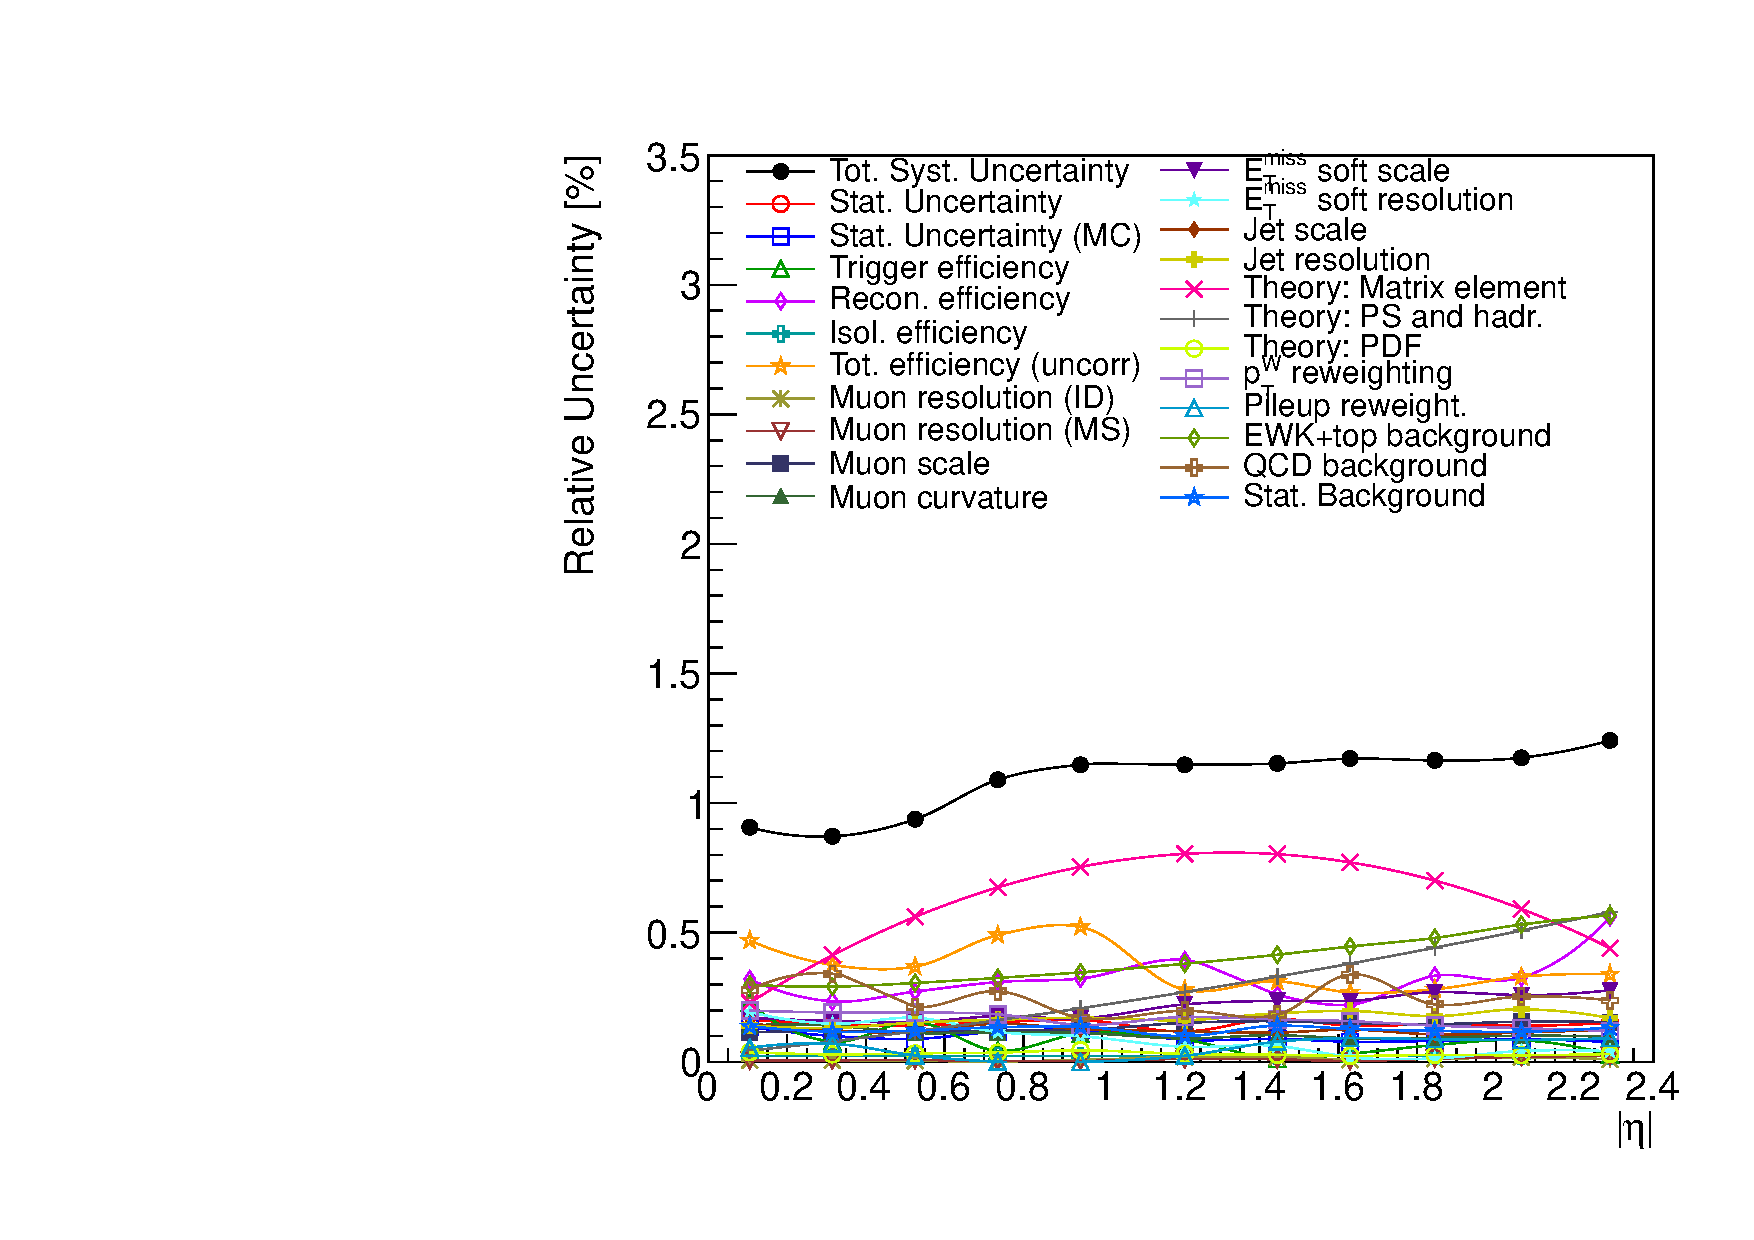
\includegraphics[width=1.0\textwidth]{dates/20130602/figures/v26.allqcd/Wmn_SYSTEM_1D_PT25_NEG_Unc_proj}
\column{.5\textwidth}

\centering
\only{ \small{ $W^{+}$: wmunu v8} }
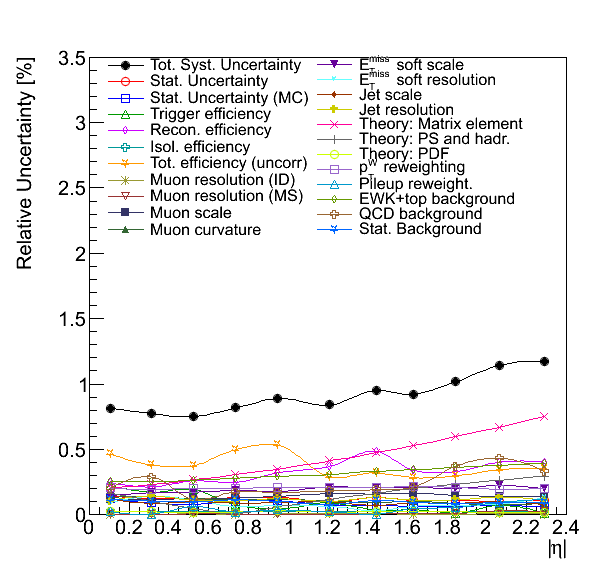
\includegraphics[width=1.0\textwidth]{dates/20130602/figures/v26.allqcd/Wmn_SYSTEM_1D_PT25_POS_Unc_proj}
\cole
}

\slide{ Double-differential uncertainties }
{
Plots of double-differential uncertainties in each pt bin.
}

\slide{ $20 < p_T < 25$ }
{
\colb[T]
\column{.5\textwidth}
\centering
\only{ \small{ $W^{-}$: wmunu v8} }
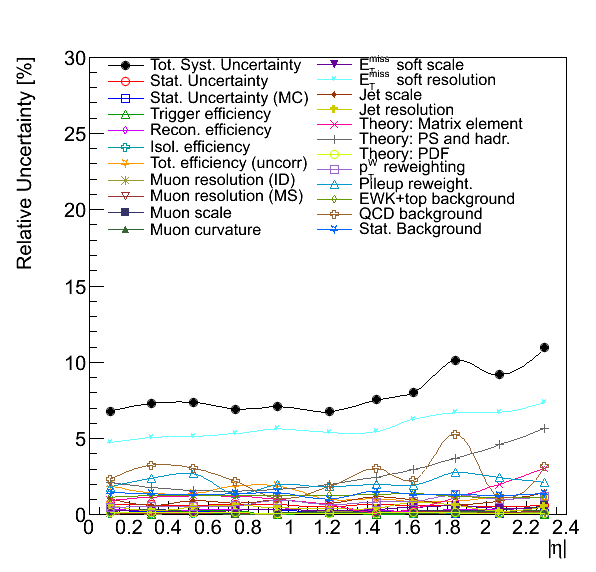
\includegraphics[width=1.0\textwidth]{dates/20130602/figures/v26.allqcd/Wmn_SYSTEM30_2D_PT20_NEG_Unc_2d_Slice_1}
\column{.5\textwidth}

\centering
\only{ \small{ $W^{+}$: wmunu v8} }
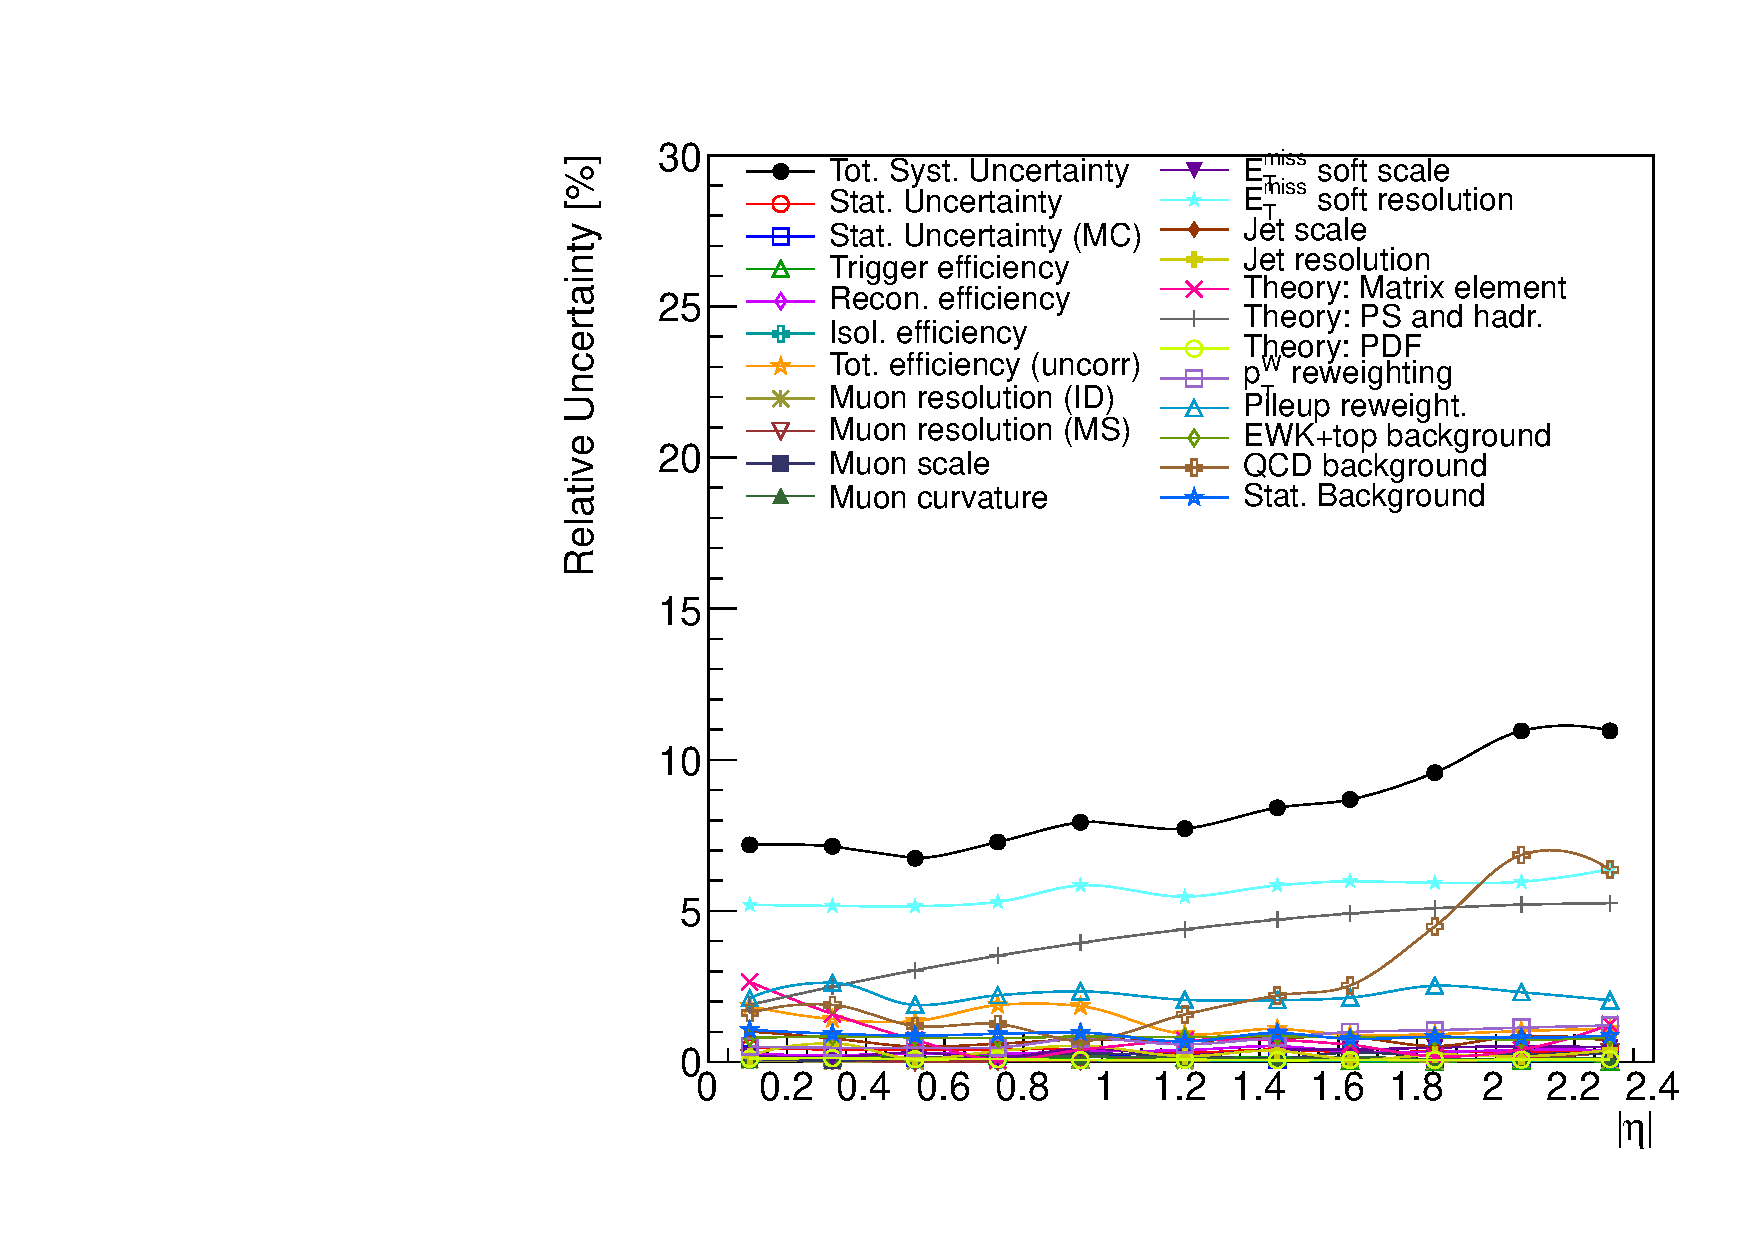
\includegraphics[width=1.0\textwidth]{dates/20130602/figures/v26.allqcd/Wmn_SYSTEM30_2D_PT20_POS_Unc_2d_Slice_1}
\cole
}

\slide{ $25 < p_T < 30$ }
{
\colb[T]
\column{.5\textwidth}
\centering
\only{ \small{ $W^{-}$: wmunu v8} }
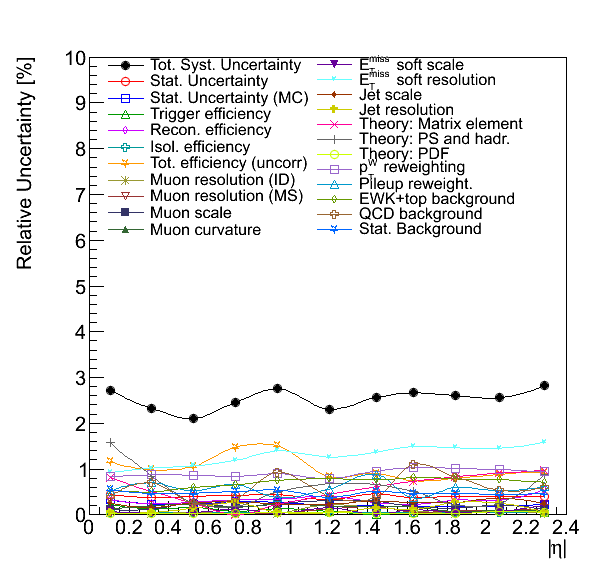
\includegraphics[width=1.0\textwidth]{dates/20130602/figures/v26.allqcd/Wmn_SYSTEM_2D_PT20_NEG_Unc_2d_Slice_2}
\column{.5\textwidth}

\centering
\only{ \small{ $W^{+}$: wmunu v8} }
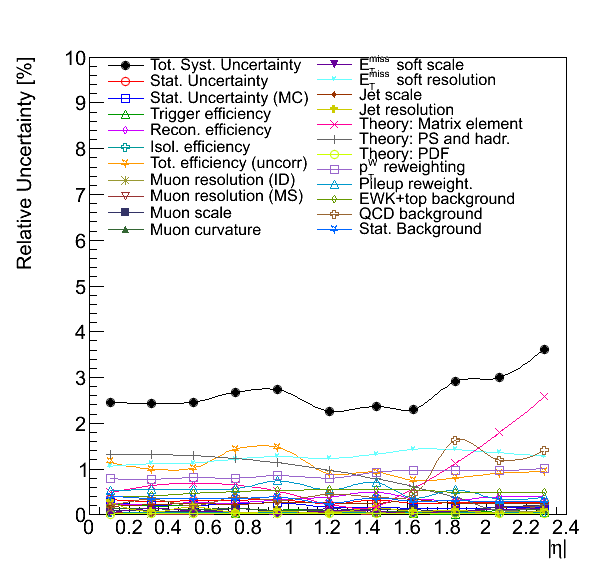
\includegraphics[width=1.0\textwidth]{dates/20130602/figures/v26.allqcd/Wmn_SYSTEM_2D_PT20_POS_Unc_2d_Slice_2}
\cole
}

\slide{ $30 < p_T < 35$ }
{
\colb[T]
\column{.5\textwidth}
\centering
\only{ \small{ $W^{-}$: wmunu v8} }
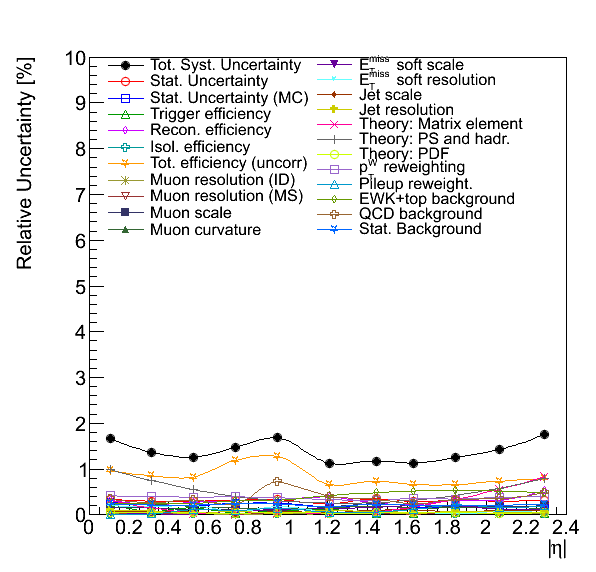
\includegraphics[width=1.0\textwidth]{dates/20130602/figures/v26.allqcd/Wmn_SYSTEM_2D_PT20_NEG_Unc_2d_Slice_3}
\column{.5\textwidth}

\centering
\only{ \small{ $W^{+}$: wmunu v8} }
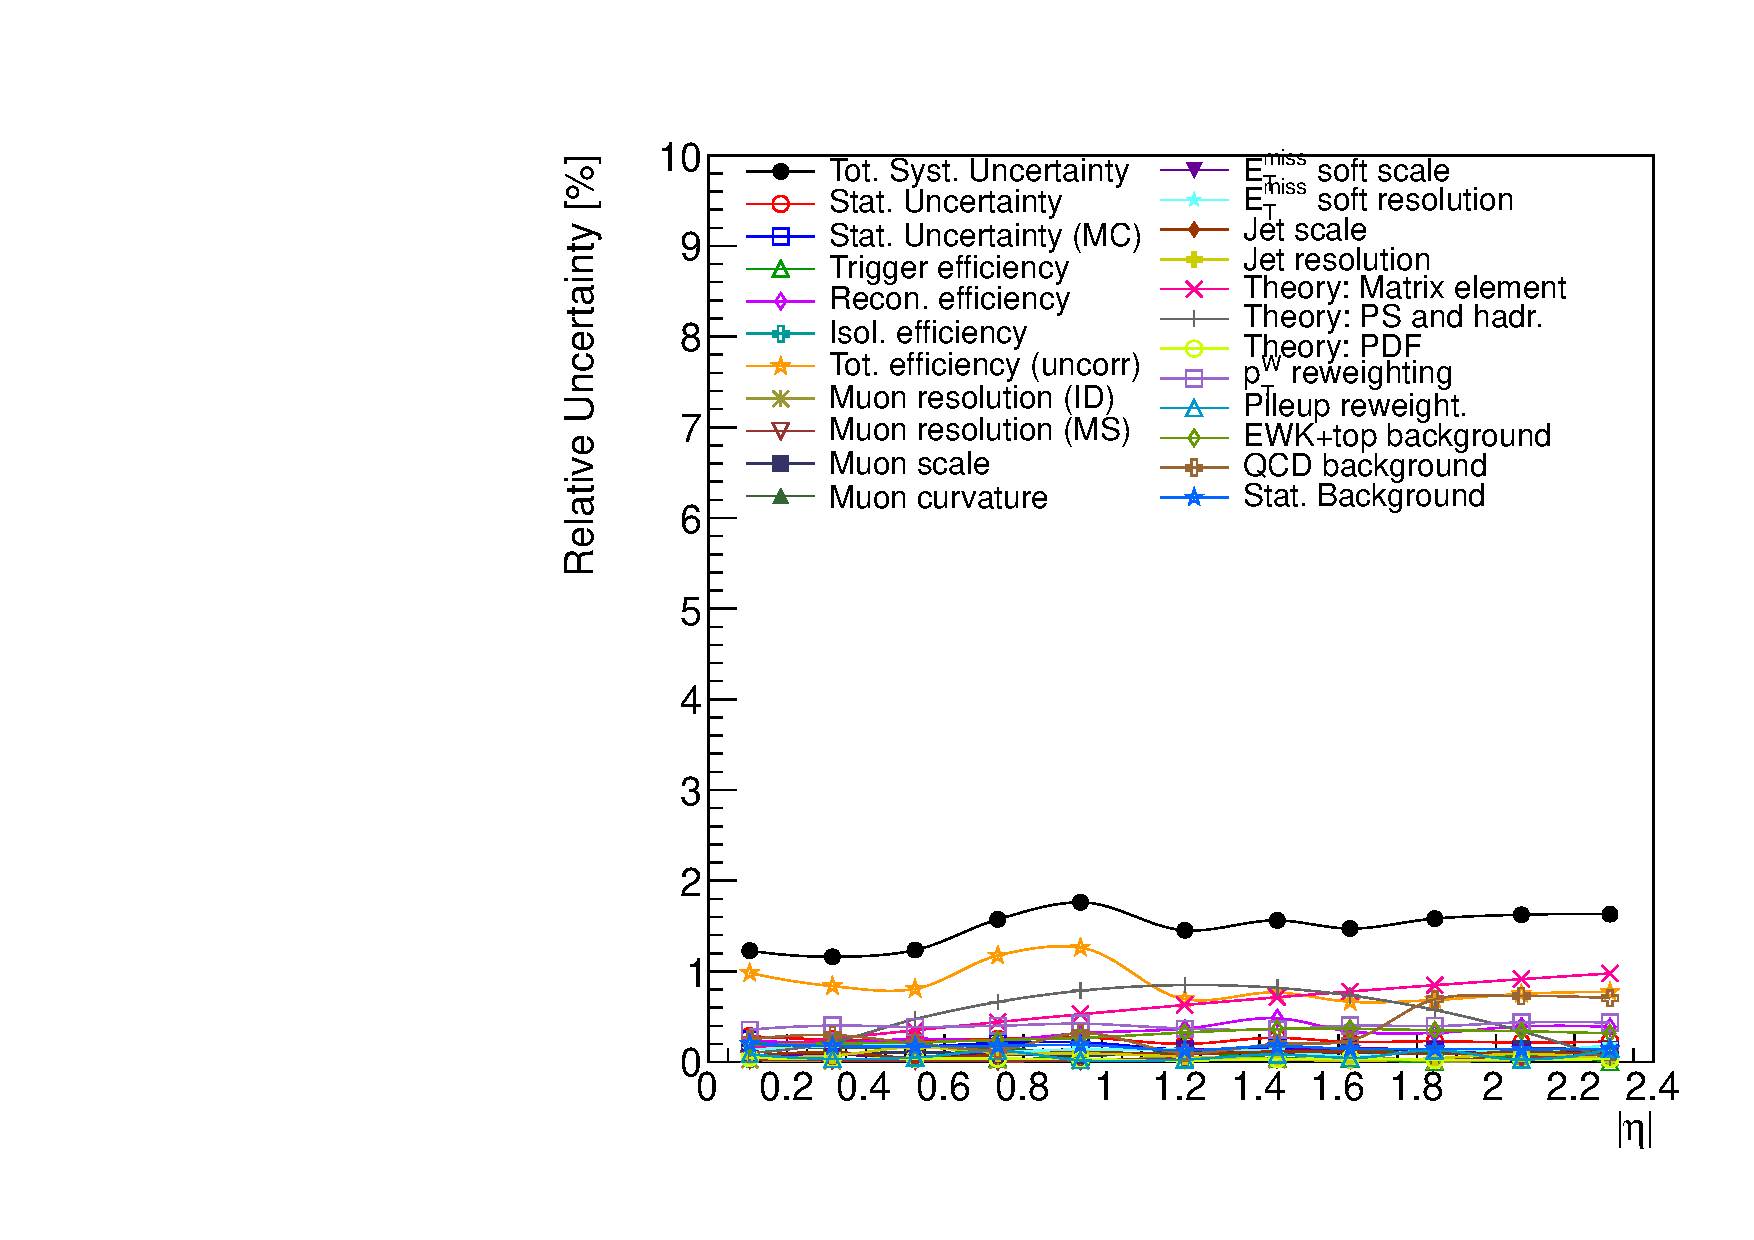
\includegraphics[width=1.0\textwidth]{dates/20130602/figures/v26.allqcd/Wmn_SYSTEM_2D_PT20_POS_Unc_2d_Slice_3}
\cole
}

\slide{ $35 < p_T < 40$ }
{
\colb[T]
\column{.5\textwidth}
\centering
\only{ \small{ $W^{-}$: wmunu v8} }
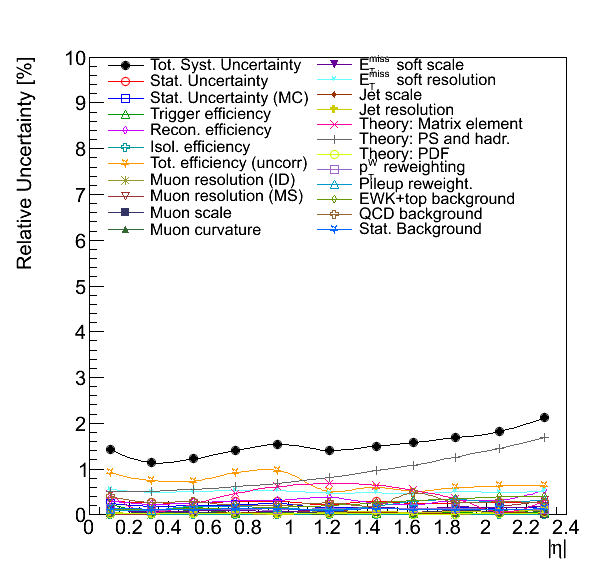
\includegraphics[width=1.0\textwidth]{dates/20130602/figures/v26.allqcd/Wmn_SYSTEM_2D_PT20_NEG_Unc_2d_Slice_4}
\column{.5\textwidth}

\centering
\only{ \small{ $W^{+}$: wmunu v8} }
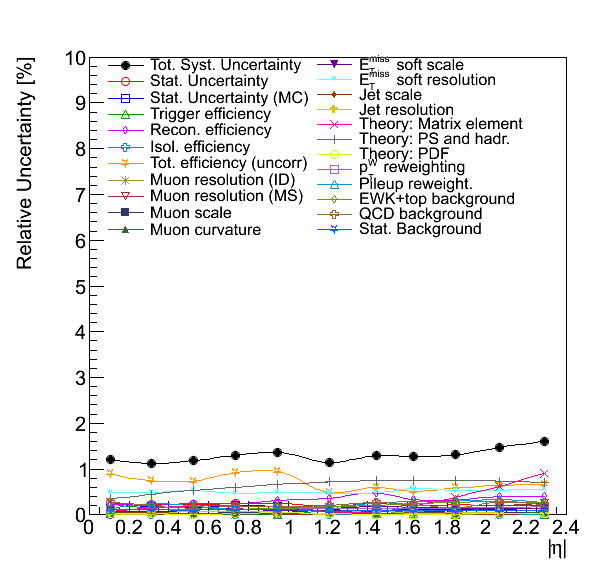
\includegraphics[width=1.0\textwidth]{dates/20130602/figures/v26.allqcd/Wmn_SYSTEM_2D_PT20_POS_Unc_2d_Slice_4}
\cole
}

\slide{ $40 < p_T < 45$ }
{
\colb[T]
\column{.5\textwidth}
\centering
\only{ \small{ $W^{-}$: wmunu v8} }
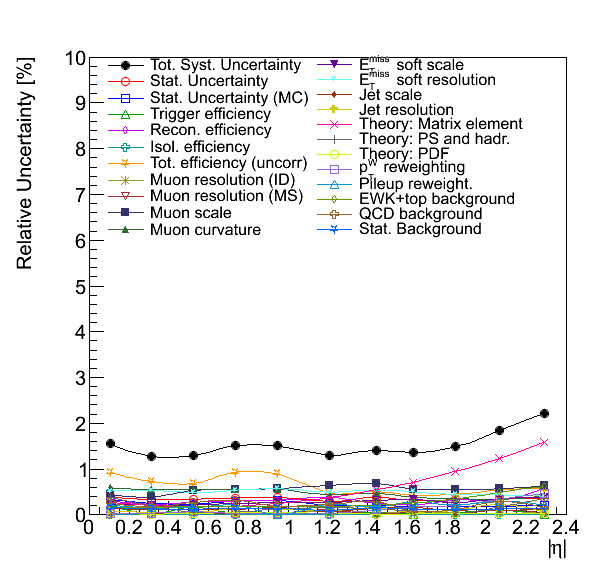
\includegraphics[width=1.0\textwidth]{dates/20130602/figures/v26.allqcd/Wmn_SYSTEM_2D_PT20_NEG_Unc_2d_Slice_5}
\column{.5\textwidth}

\centering
\only{ \small{ $W^{+}$: wmunu v8} }
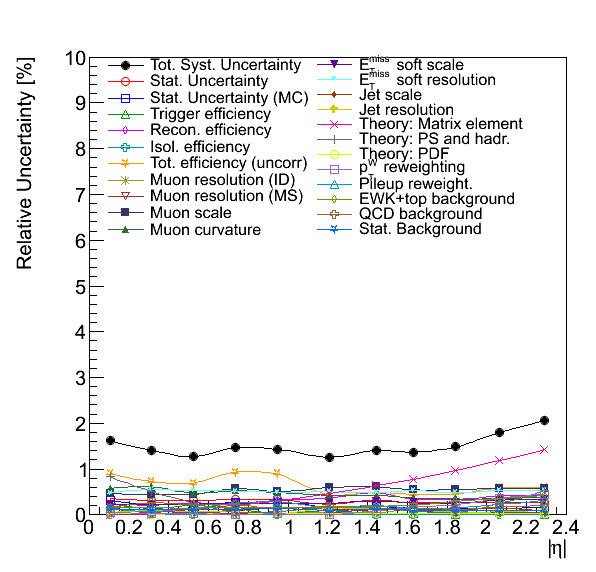
\includegraphics[width=1.0\textwidth]{dates/20130602/figures/v26.allqcd/Wmn_SYSTEM_2D_PT20_POS_Unc_2d_Slice_5}
\cole
}

\slide{ $45 < p_T < 50$ }
{
\colb[T]
\column{.5\textwidth}
\centering
\only{ \small{ $W^{-}$: wmunu v8} }
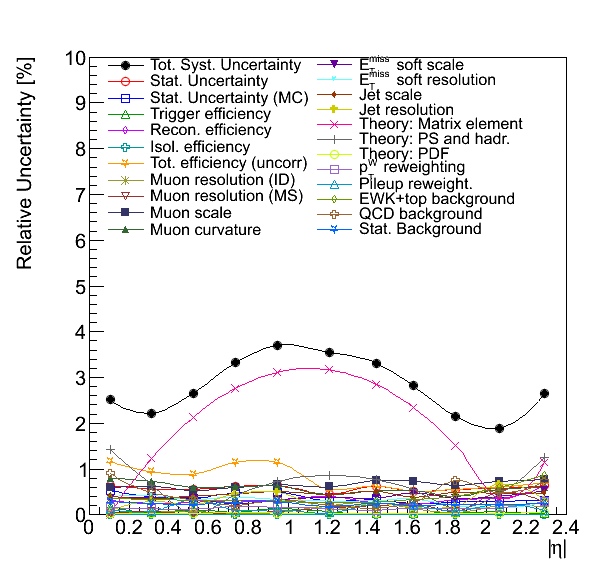
\includegraphics[width=1.0\textwidth]{dates/20130602/figures/v26.allqcd/Wmn_SYSTEM_2D_PT20_NEG_Unc_2d_Slice_6}
\column{.5\textwidth}

\centering
\only{ \small{ $W^{+}$: wmunu v8} }
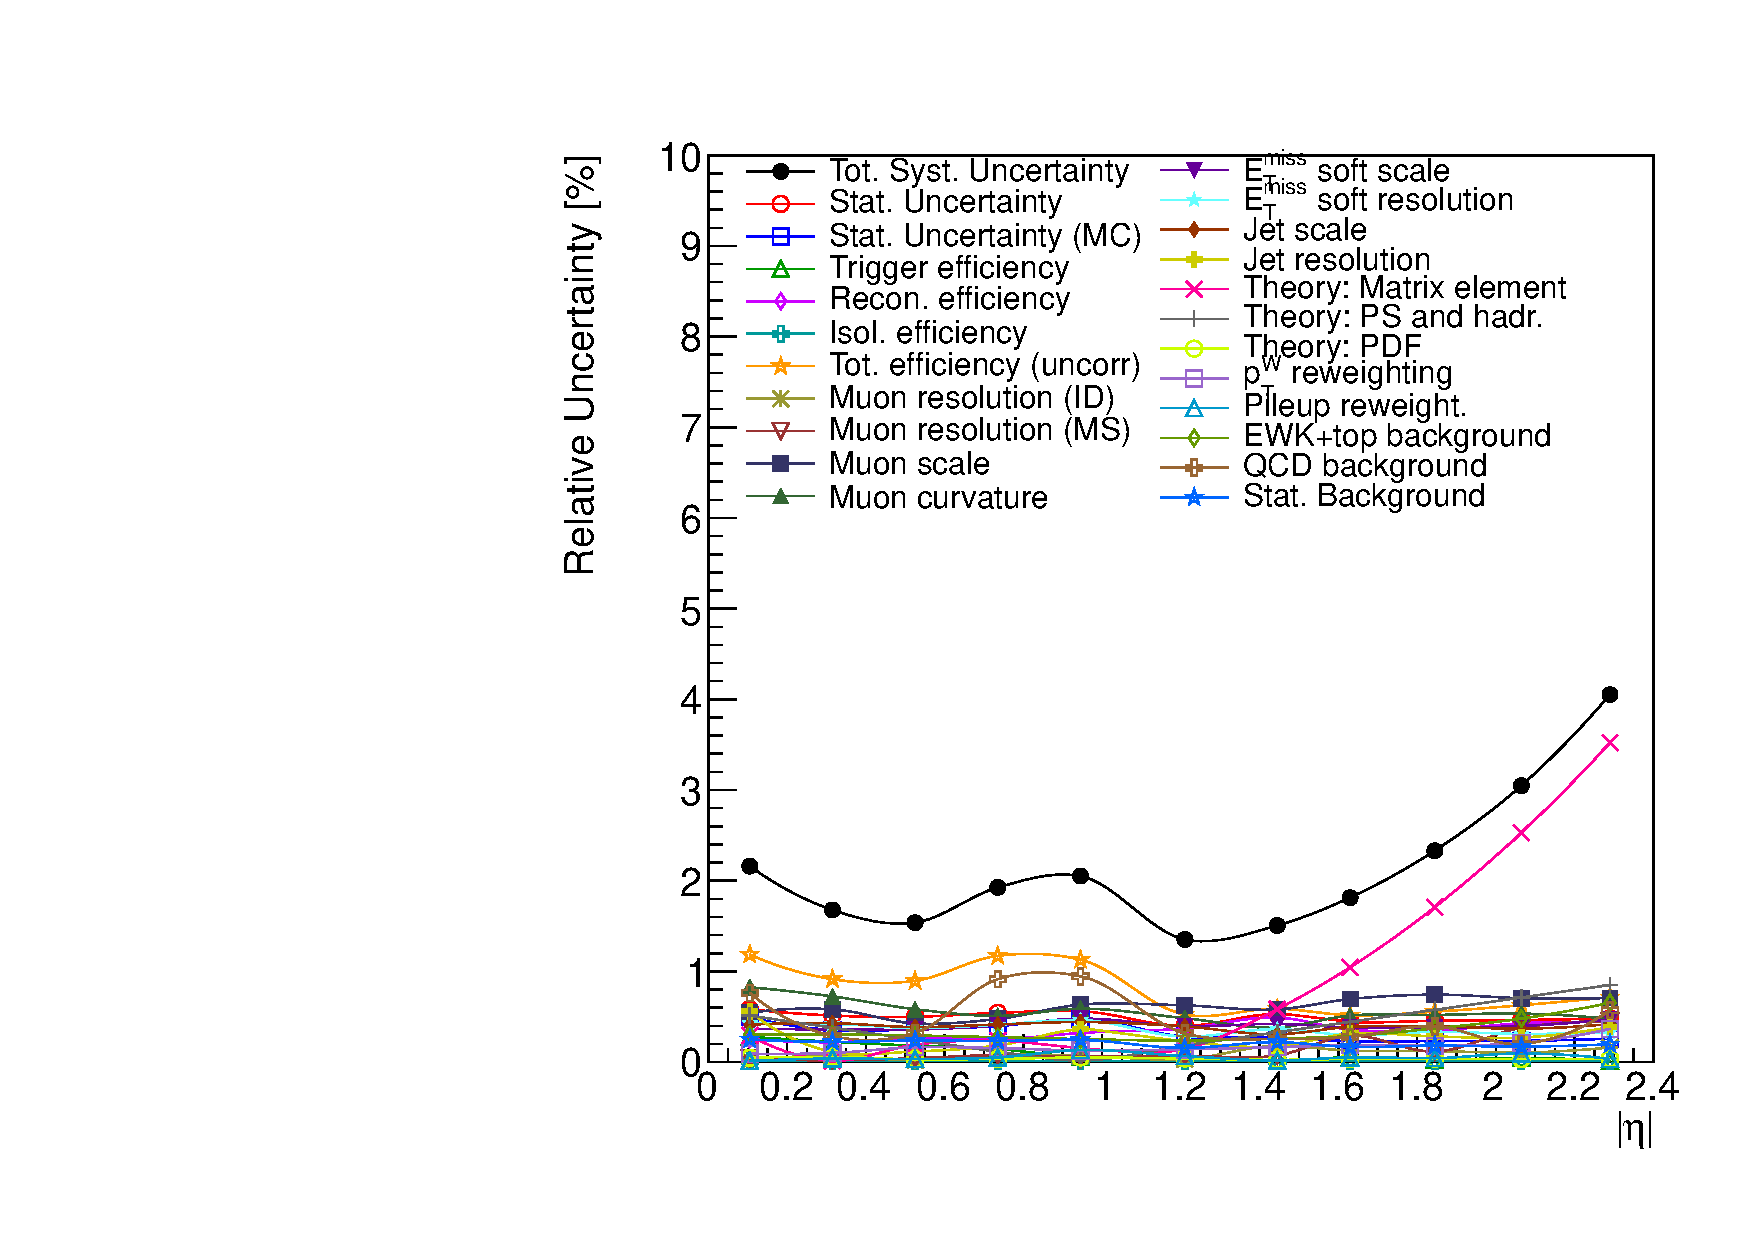
\includegraphics[width=1.0\textwidth]{dates/20130602/figures/v26.allqcd/Wmn_SYSTEM_2D_PT20_POS_Unc_2d_Slice_6}
\cole
}

\slide{ $p_T > 50$ }
{
\colb[T]
\column{.5\textwidth}
\centering
\only{ \small{ $W^{-}$: wmunu v8} }
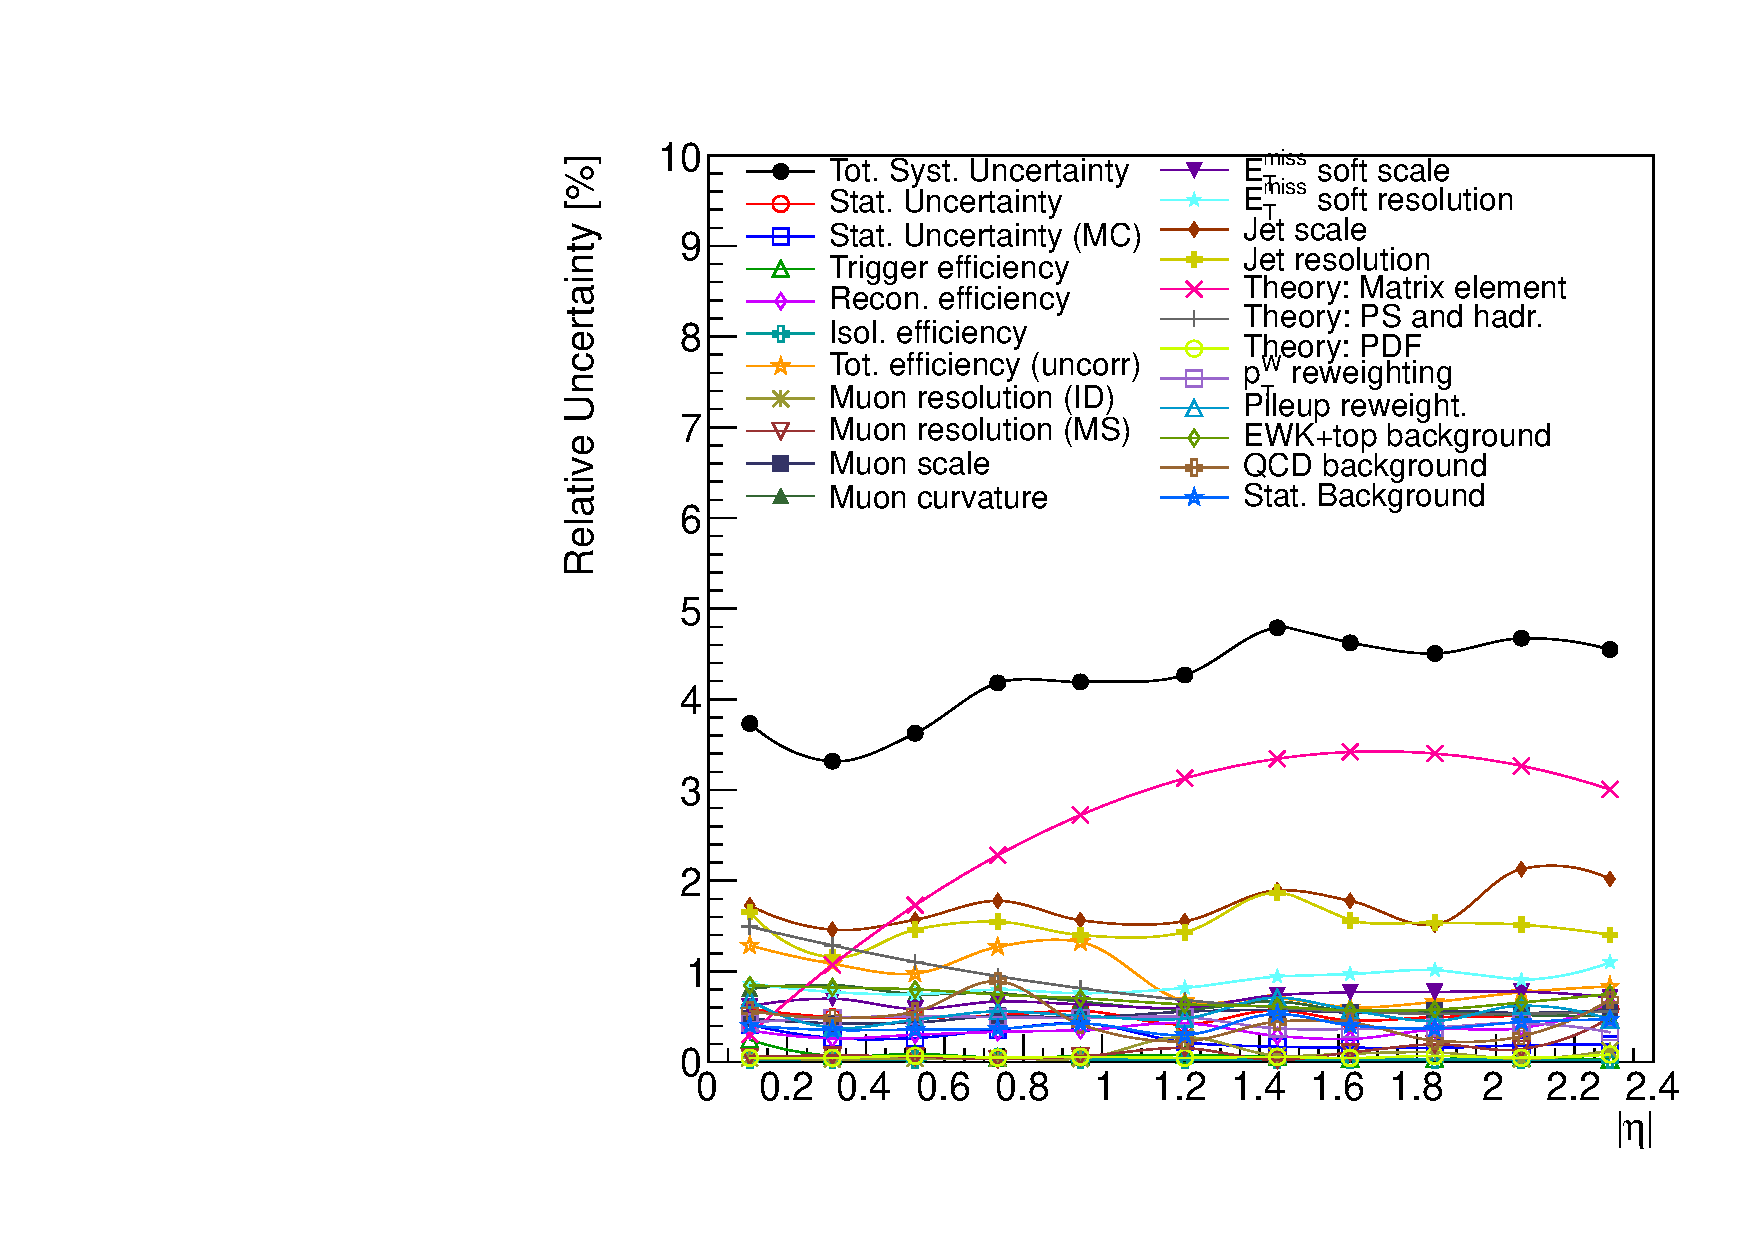
\includegraphics[width=1.0\textwidth]{dates/20130602/figures/v26.allqcd/Wmn_SYSTEM_2D_PT20_NEG_Unc_2d_Slice_7}
\column{.5\textwidth}

\centering
\only{ \small{ $W^{+}$: wmunu v8} }
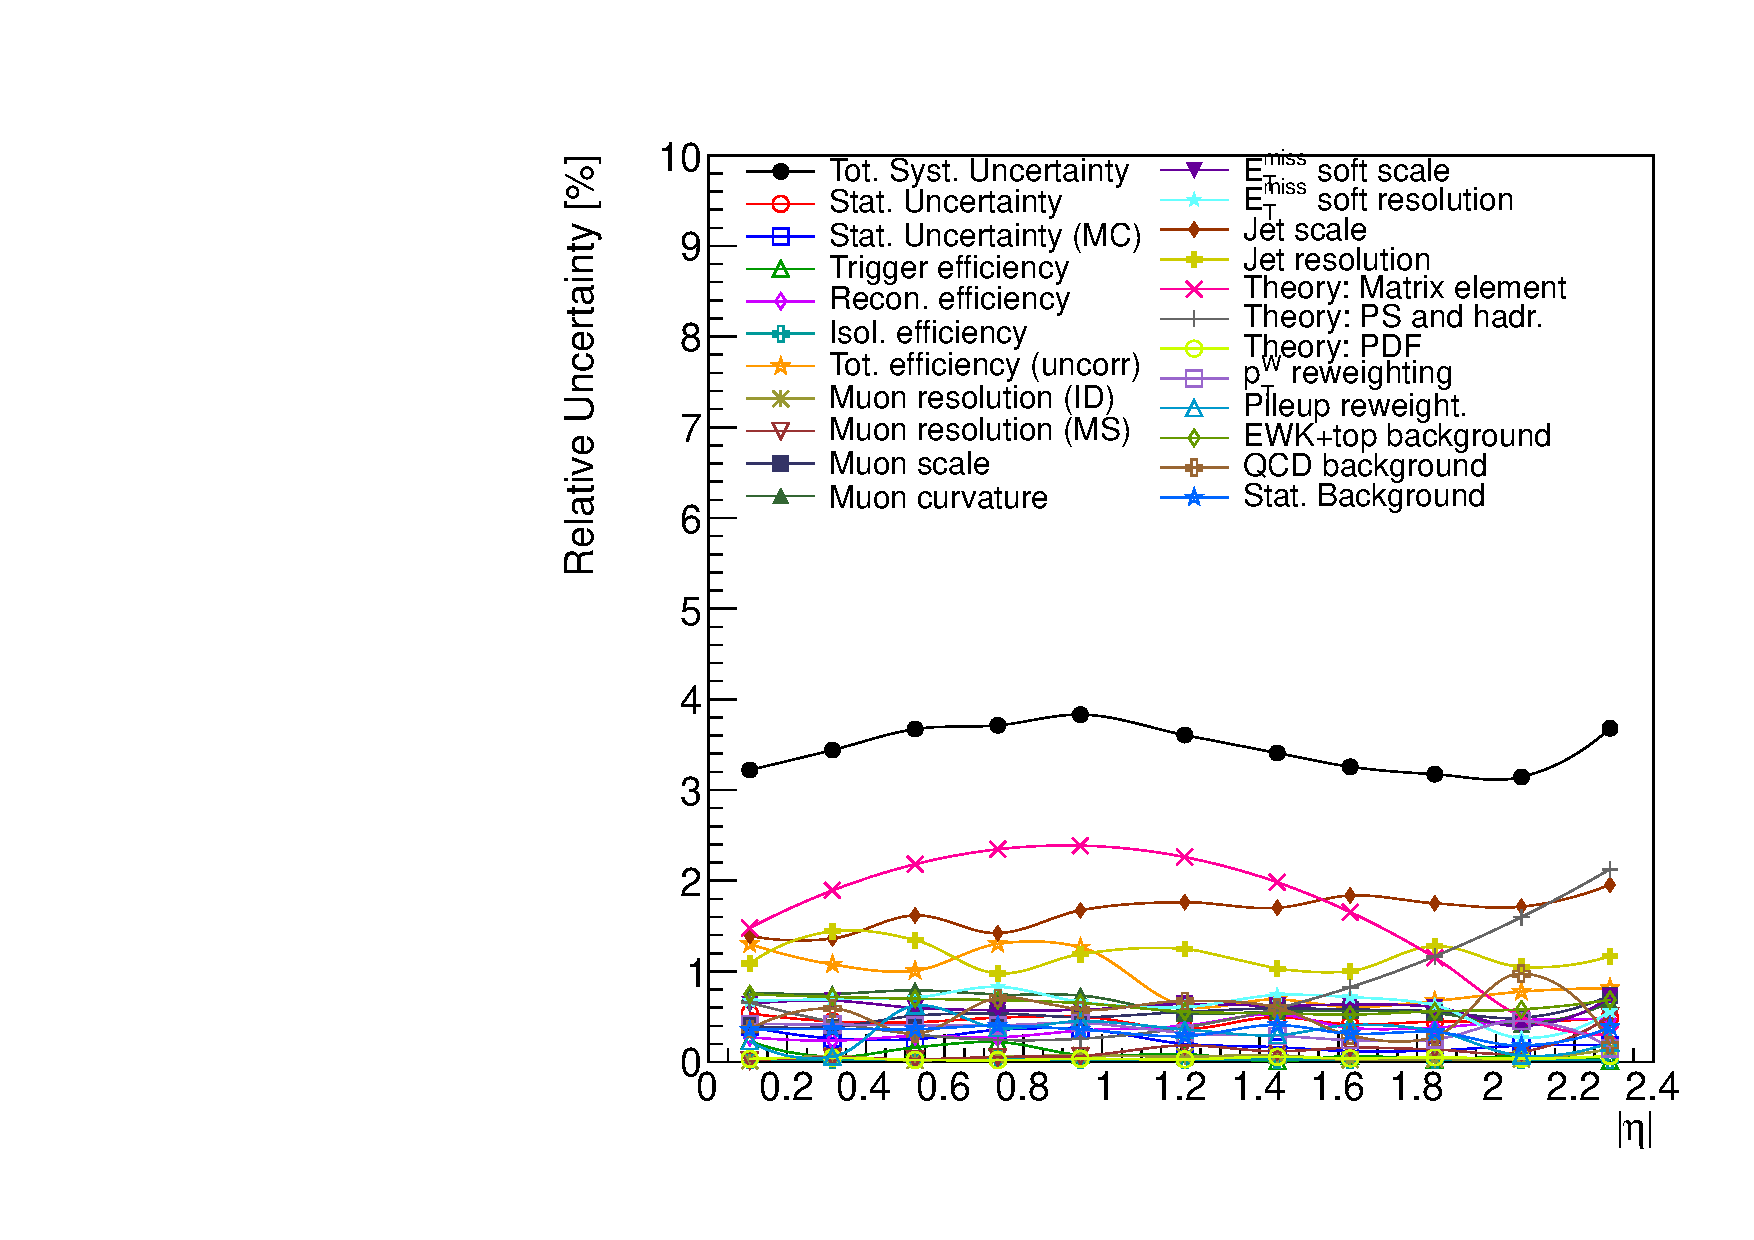
\includegraphics[width=1.0\textwidth]{dates/20130602/figures/v26.allqcd/Wmn_SYSTEM_2D_PT20_POS_Unc_2d_Slice_7}
\cole
}


\slide{ Compare with: single-differential wenu ($pt>25$ GeV)}
{
\colb[T]
\column{.5\textwidth}
\centering
\small{ $W^{-}$: wenu}
\includegraphics[width=1.0\textwidth]{/home/antonk/SupportingDocument/Wenu/figures/uncert/with_theory/Wenu_Unc_neg}
\column{.5\textwidth}

\centering
\small{ $W^{+}$: wenu}
\includegraphics[width=1.0\textwidth]{/home/antonk/SupportingDocument/Wenu/figures/uncert/with_theory/Wenu_Unc_pos}
\cole
}
